\section{Contextualização da atividade}

Considerando o sistema de 5 barras da Figura \ref{sistemaparte2}, implementou-se um programa computacional para calcular os fluxos de potência entre as linhas do sistema. Utilizou-se o fluxo de potência linearizado. Para cada cenário, determinou-se os fluxos de potência (em p.u.) entre as linhas e apresentou-se na forma de tabela destacando os casos em que houveram violações nas restrições (fluxos superiores a 1,0 p.u.). Nos casos em que houver acréscimo de carga, considerou-se que o acréscimo da geração deverá ser realizado pelo gerador conectado a \textbf{barra 1}.

A Tabela \ref{part2:dadossist} refere-se aos dados do sistema proposto que será analisado neste problema.

\begin{table}[!h]
\centering
\caption{Dados do sistema proposto}
\label{part2:dadossist}
\begin{tabular}{|c|c|c|c|c|}
\hline
\multirow{2}{*}{\textbf{Linha}} & \multicolumn{2}{c|}{\textbf{Barra}} & \multirow{2}{*}{\textbf{R (p.u.)}} & \multirow{2}{*}{\textbf{X (p.u.)}} \\ \cline{2-3}
 & \textbf{De} & \textbf{Para} &  &  \\ \hline
\textit{\textbf{1}} & \textit{1} & \textit{2} & 0,10 & 0,40 \\ \hline
\textit{\textbf{2}} & \textit{1} & \textit{4} & 0,15 & 0,60 \\ \hline
\textit{\textbf{3}} & \textit{1} & \textit{5} & 0,05 & 0,20 \\ \hline
\textit{\textbf{4}} & \textit{2} & \textit{3} & 0,05 & 0,20 \\ \hline
\textit{\textbf{5}} & \textit{2} & \textit{4} & 0,10 & 0,40 \\ \hline
\textit{\textbf{6}} & \textit{3} & \textit{5} & 0,05 & 0,20 \\ \hline
\end{tabular}
\end{table}

A Tabela \ref{part2:dadossist2} refere-se aos dados de carga e geração do mesmo sistema.

\begin{table}[!h]
\centering
\caption{Dados de geração e carga do sistema}
\label{part2:dadossist2}
\begin{tabular}{|c|c|c|}
\hline
\textbf{Barra} & \textbf{Carga (p.u.)} & \textbf{Geração (p.u.)} \\ \hline
\textit{\textbf{1}} & \textit{0,240} & \textit{1,130} \\ \hline
\textit{\textbf{2}} & \textit{0,720} & \textit{0,500} \\ \hline
\textit{\textbf{3}} & \textit{0,120} & \textit{0,650} \\ \hline
\textit{\textbf{4}} & \textit{0,480} & \textit{-} \\ \hline
\textit{\textbf{5}} & \textit{0,720} & \textit{-} \\ \hline
\end{tabular}
\end{table}

A representação unifilar do sistema proposto para este problema está representada na Figura \ref{sistemaparte2}.

\begin{figure}[!h]
	\centering
	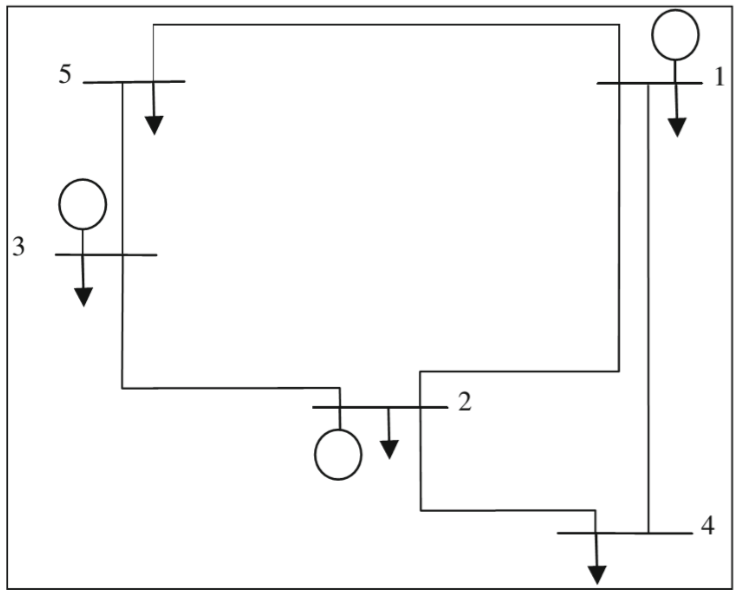
\includegraphics[scale=0.35]{fig1part2}
	\caption{Sistema proposto de cinco barras}
	\label{sistemaparte2}
\end{figure}

\section{Resolução do problema proposto}

	Todos os cálculos referentes a esta solução foram efetuados no \textit{software} MATLAB®

\subsection{Equacionamento e definição de métodos}

	O procedimento a ser definido para o cálculo do fluxo de potência em cada linha do sistema é o mesmo utilizado na primeira parte da atividade prática supervisionada, conforme a Sessão 1.1 apresenta. Ou seja, será utilizado o método linearizado para o cálculo do fluxo de potência.

\subsection{Cálculo dos parâmetros}
	
	Implementado o algoritmo que faz o estudo de fluxo linearizado do sistema apresentado na Figura \ref{sistemaparte2}, obteve-se as seguintes respostas para cada cenário apresentado, conforme solicitado no roteiro da atividade prática supervisionada: Caso sem contingência, contingência em cada linha ($n-1$) e contingência em cada linha com carga extra ($n-1$). 
	
	O código efetuado em MATLAB® encontra-se anexo a este documento.
	
\subsubsection{Valores das tensões e fluxos de potência obtidos no MATLAB®}
\begin{verbatim}
Código implementado em MATLAB por Rafael Bonotto e Raphael Machado.
Planejamento de Sistemas Energéticos - APS 02 - Parte 2

[1] - Considere o caso base (sem contingência)
[2] - Contingência em cada linha (N - 1)
[3] - Contingência em cada linha (N – 1) com carga extra (%)
=======================================================================
Cenário: 1
======Teta=======Valores======
    1.0000         0
    2.0000   -0.1528
    3.0000   -0.0565
    4.0000   -0.3221
    5.0000   -0.1723

Fluxo de Potência na Linha 1-2(sem contingência):     0.1910
Fluxo de Potência na Linha 1-4(sem contingência):     0.2684
Fluxo de Potência na Linha 1-5(sem contingência):     0.4306
Fluxo de Potência na Linha 2-3(sem contingência):    -0.2406
Fluxo de Potência na Linha 2-4(sem contingência):     0.2116
Fluxo de Potência na Linha 3-5(sem contingência):     0.2894
=======================================================================





Cenário: 2
Linha 1 - 2 em Falta
======Teta=======Valores======
    1.0000         0
    2.0000   -0.5920
    3.0000   -0.3040
    4.0000   -0.8160
    5.0000   -0.4400

Fluxo da Linha 1-2 com contingência da Linha 1-2:      0
Fluxo da Linha 1-4 com contingência da Linha 1-2:     0.3400
Fluxo da Linha 1-5 com contingência da Linha 1-2:     0.5500
Fluxo da Linha 2-3 com contingência da Linha 1-2:    -0.3600
Fluxo da Linha 2-4 com contingência da Linha 1-2:     0.1400
Fluxo da Linha 3-5 com contingência da Linha 1-2:     0.1700

Linha 1 - 4 em Falta
======Teta=======Valores======
    1.0000         0
    2.0000   -0.5632
    3.0000   -0.2848
    4.0000   -1.3312
    5.0000   -0.4304

Fluxo da Linha 1-2 com contingência da Linha 1-4:     0.3520
Fluxo da Linha 1-4 com contingência da Linha 1-4:      0
Fluxo da Linha 1-5 com contingência da Linha 1-4:     0.5380
Fluxo da Linha 2-3 com contingência da Linha 1-4:    -0.3480
Fluxo da Linha 2-4 com contingência da Linha 1-4:     0.4800
Fluxo da Linha 3-5 com contingência da Linha 1-4:     0.1820

Linha 1 - 5 em Falta
======Teta=======Valores======
    1.0000         0
    2.0000   -0.7977
    3.0000   -0.9497
    4.0000   -0.9394
    5.0000   -1.5257
Fluxo da Linha 1-2 com contingência da Linha 1-5:     0.4986
Fluxo da Linha 1-4 com contingência da Linha 1-5:     0.3914
Fluxo da Linha 1-5 com contingência da Linha 1-5:      0
Fluxo da Linha 2-3 com contingência da Linha 1-5:     0.1900
Fluxo da Linha 2-4 com contingência da Linha 1-5:     0.0886
Fluxo da Linha 3-5 com contingência da Linha 1-5:     0.7200

Linha 2 - 3 em Falta
======Teta=======Valores======
    1.0000         0
    2.0000   -0.5806
    3.0000    0.2720
    4.0000   -0.8091
    5.0000   -0.1520
Fluxo da Linha 1-2 com contingência da Linha 2-3:     0.3629
Fluxo da Linha 1-4 com contingência da Linha 2-3:     0.3371
Fluxo da Linha 1-5 com contingência da Linha 2-3:     0.1900
Fluxo da Linha 2-3 com contingência da Linha 2-3:      0
Fluxo da Linha 2-4 com contingência da Linha 2-3:     0.1429
Fluxo da Linha 3-5 com contingência da Linha 2-3:     0.5300

Linha 2 - 4 em Falta
======Teta=======Valores======
    1.0000         0
    2.0000   -0.1024
    3.0000    0.0224
    4.0000   -1.1520
    5.0000   -0.2768
Fluxo da Linha 1-2 com contingência da Linha 2-4:     0.0640
Fluxo da Linha 1-4 com contingência da Linha 2-4:     0.4800
Fluxo da Linha 1-5 com contingência da Linha 2-4:     0.3460
Fluxo da Linha 2-3 com contingência da Linha 2-4:    -0.1560
Fluxo da Linha 2-4 com contingência da Linha 2-4:      0
Fluxo da Linha 3-5 com contingência da Linha 2-4:     0.3740

Linha 3 - 5 em Falta
======Teta=======Valores======
    1.0000         0
    2.0000    0.0251
    3.0000    0.4491
    4.0000   -0.4457
    5.0000   -0.5760
Fluxo da Linha 1-2 com contingência da Linha 3-5:    -0.0157
Fluxo da Linha 1-4 com contingência da Linha 3-5:     0.1857
Fluxo da Linha 1-5 com contingência da Linha 3-5:     0.7200
Fluxo da Linha 2-3 com contingência da Linha 3-5:    -0.5300
Fluxo da Linha 2-4 com contingência da Linha 3-5:     0.2943
Fluxo da Linha 3-5 com contingência da Linha 3-5:      0

=======================================================================
Escolha o cenário: 3
Escolha o valor de carga extra (em porcentagem): 50

Linha de Falta 1 - 2
======Teta=======Valores======
    1.0000         0
    2.0000   -1.5880
    3.0000   -1.0960
    4.0000   -1.6440
    5.0000   -0.9800
Fluxo de Potência da Linha 1-2 com contingência da Linha 1-2:      0
Fluxo de Potência da Linha 1-4 com contingência da Linha 1-2:     0.6850
Fluxo de Potência da Linha 1-5 com contingência da Linha 1-2:     1.2250
Fluxo de Potência da Linha 2-3 com contingência da Linha 1-2:    -0.6150
Fluxo de Potência da Linha 2-4 com contingência da Linha 1-2:     0.0350
Fluxo de Potência da Linha 3-5 com contingência da Linha 1-2:    -0.1450

Linha de Falta 1 - 4
======Teta=======Valores======
    1.0000         0
    2.0000   -2.5856
    3.0000   -1.7984
    4.0000   -4.8896
    5.0000   -1.7632
Fluxo de Potência da Linha 1-2 com contingência da Linha 1-4:     0.8080
Fluxo de Potência da Linha 1-4 com contingência da Linha 1-4:      0
Fluxo de Potência da Linha 1-5 com contingência da Linha 1-4:     1.1020
Fluxo de Potência da Linha 2-3 com contingência da Linha 1-4:    -0.4920
Fluxo de Potência da Linha 2-4 com contingência da Linha 1-4:     0.7200
Fluxo de Potência da Linha 3-5 com contingência da Linha 1-4:    -0.0220

Linha de Falta 1 - 5
======Teta=======Valores======
    1.0000         0
    2.0000   -3.7074
    3.0000   -4.6834
    4.0000   -3.6069
    5.0000   -6.4114
Fluxo de Potência da Linha 1-2 com contingência da Linha 1-5:     1.1586
Fluxo de Potência da Linha 1-4 com contingência da Linha 1-5:     0.7514
Fluxo de Potência da Linha 1-5 com contingência da Linha 1-5:      0
Fluxo de Potência da Linha 2-3 com contingência da Linha 1-5:     0.6100
Fluxo de Potência da Linha 2-4 com contingência da Linha 1-5:    -0.0314
Fluxo de Potência da Linha 3-5 com contingência da Linha 1-5:     1.0800

Linha de Falta 2 - 3
======Teta=======Valores======
    1.0000         0
    2.0000   -2.3131
    3.0000   -0.2240
    4.0000   -2.7703
    5.0000   -0.9760
Fluxo de Potência da Linha 1-2 com contingência da Linha 2-3:     0.7229
Fluxo de Potência da Linha 1-4 com contingência da Linha 2-3:     0.5771
Fluxo de Potência da Linha 1-5 com contingência da Linha 2-3:     0.6100
Fluxo de Potência da Linha 2-3 com contingência da Linha 2-3:      0
Fluxo de Potência da Linha 2-4 com contingência da Linha 2-3:     0.1429
Fluxo de Potência da Linha 3-5 com contingência da Linha 2-3:     0.4700

Linha de Falta 2 - 4
======Teta=======Valores======
    1.0000         0
    2.0000   -1.2032
    3.0000   -0.8768
    4.0000   -3.4560
    5.0000   -1.3024
Fluxo de Potência da Linha 1-2 com contingência da Linha 2-4:     0.3760
Fluxo de Potência da Linha 1-4 com contingência da Linha 2-4:     0.7200
Fluxo de Potência da Linha 1-5 com contingência da Linha 2-4:     0.8140
Fluxo de Potência da Linha 2-3 com contingência da Linha 2-4:    -0.2040
Fluxo de Potência da Linha 2-4 com contingência da Linha 2-4:      0
Fluxo de Potência da Linha 3-5 com contingência da Linha 2-4:     0.2660

Linha de Falta 3 - 5
======Teta=======Valores======
    1.0000         0
    2.0000   -1.2389
    3.0000   -0.4869
    4.0000   -2.1257
    5.0000   -1.7280
Fluxo de Potência da Linha 1-2 com contingência da Linha 3-5:     0.3871
Fluxo de Potência da Linha 1-4 com contingência da Linha 3-5:     0.4429
Fluxo de Potência da Linha 1-5 com contingência da Linha 3-5:     1.0800
Fluxo de Potência da Linha 2-3 com contingência da Linha 3-5:    -0.4700
Fluxo de Potência da Linha 2-4 com contingência da Linha 3-5:     0.2771
Fluxo de Potência da Linha 3-5 com contingência da Linha 3-5:      0

=======================================================================





Cenário: 3
Escolha o valor de carga extra(em porcentagem): 150

Linha de Falta 1 - 2
======Teta=======Valores======
    1.0000         0
    2.0000   -3.5800
    3.0000   -2.6800
    4.0000   -3.3000
    5.0000   -2.0600
Fluxo de Potência da Linha 1-2 com contingência da Linha 1-2:      0
Fluxo de Potência da Linha 1-4 com contingência da Linha 1-2:     1.3750
Fluxo de Potência da Linha 1-5 com contingência da Linha 1-2:     2.5750
Fluxo de Potência da Linha 2-3 com contingência da Linha 1-2:    -1.1250
Fluxo de Potência da Linha 2-4 com contingência da Linha 1-2:    -0.1750
Fluxo de Potência da Linha 3-5 com contingência da Linha 1-2:    -0.7750

Linha de Falta 1 - 4
======Teta=======Valores======
    1.0000         0
    2.0000   -5.5040
    3.0000   -4.2560
    4.0000   -9.3440
    5.0000   -3.5680
Fluxo de Potência da Linha 1-2 com contingência da Linha 1-4:     1.7200
Fluxo de Potência da Linha 1-4 com contingência da Linha 1-4:      0
Fluxo de Potência da Linha 1-5 com contingência da Linha 1-4:     2.2300
Fluxo de Potência da Linha 2-3 com contingência da Linha 1-4:    -0.7800
Fluxo de Potência da Linha 2-4 com contingência da Linha 1-4:     1.2000
Fluxo de Potência da Linha 3-5 com contingência da Linha 1-4:    -0.4300

Linha de Falta 1 - 5
======Teta=======Valores======
    1.0000         0
    2.0000   -7.9314
    3.0000  -10.2514
    4.0000   -7.0629
    5.0000  -13.1314
Fluxo de Potência da Linha 1-2 com contingência da Linha 1-5:     2.4786
Fluxo de Potência da Linha 1-4 com contingência da Linha 1-5:     1.4714
Fluxo de Potência da Linha 1-5 com contingência da Linha 1-5:      0
Fluxo de Potência da Linha 2-3 com contingência da Linha 1-5:     1.4500
Fluxo de Potência da Linha 2-4 com contingência da Linha 1-5:    -0.2714
Fluxo de Potência da Linha 3-5 com contingência da Linha 1-5:     1.8000
Linha de Falta 2 - 3
======Teta=======Valores======
    1.0000         0
    2.0000   -4.6171
    3.0000   -1.7600
    4.0000   -5.0743
    5.0000   -2.3200
Fluxo de Potência da Linha 1-2 com contingência da Linha 2-3:     1.4429
Fluxo de Potência da Linha 1-4 com contingência da Linha 2-3:     1.0571
Fluxo de Potência da Linha 1-5 com contingência da Linha 2-3:     1.4500
Fluxo de Potência da Linha 2-3 com contingência da Linha 2-3:      0
Fluxo de Potência da Linha 2-4 com contingência da Linha 2-3:     0.1429
Fluxo de Potência da Linha 3-5 com contingência da Linha 2-3:     0.3500

Linha de Falta 2 - 4
======Teta=======Valores======
    1.0000         0
    2.0000   -3.2000
    3.0000   -2.7200
    4.0000   -5.7600
    5.0000   -2.8000
Fluxo de Potência da Linha 1-2 com contingência da Linha 2-4:     1.0000
Fluxo de Potência da Linha 1-4 com contingência da Linha 2-4:     1.2000
Fluxo de Potência da Linha 1-5 com contingência da Linha 2-4:     1.7500
Fluxo de Potência da Linha 2-3 com contingência da Linha 2-4:    -0.3000
Fluxo de Potência da Linha 2-4 com contingência da Linha 2-4:      0
Fluxo de Potência da Linha 3-5 com contingência da Linha 2-4:     0.0500

Linha de Falta 3 - 5
======Teta=======Valores======
    1.0000         0
    2.0000   -3.8171
    3.0000   -3.2571
    4.0000   -4.5943
    5.0000   -2.8800
Fluxo de Potência da Linha 1-2 com contingência da Linha 3-5:     1.1929
Fluxo de Potência da Linha 1-4 com contingência da Linha 3-5:     0.9571
Fluxo de Potência da Linha 1-5 com contingência da Linha 3-5:     1.8000
Fluxo de Potência da Linha 2-3 com contingência da Linha 3-5:    -0.3500
Fluxo de Potência da Linha 2-4 com contingência da Linha 3-5:     0.2429
Fluxo de Potência da Linha 3-5 com contingência da Linha 3-5:      0
\end{verbatim}
